\section{Switch OS}
This section turns to the software that runs on the switch itself. A defining property of the bare-metal switches introduced in Section~\ref{sec:basic-architecture} is that hardware and software are no longer sold as a single vertically integrated unit: using the ONIE bootloader, the operator can install any compatible Switch OS on any bare-metal switch, much as an operating system of choice is installed on a commodity server~\cite{onie, systemsapproach}.

The analogy to a server extends to the hardware itself. A Linux server always provides a general-purpose processor, with its registers, memory, and I/O, before any operating system is loaded onto it. A bare-metal switch is built the same way: it contains a conventional CPU on which the Switch OS runs, complemented by a switching chip that acts as a packet-forwarding accelerator~\cite{systemsapproach}. The relationship between the two is closely analogous to that between a CPU and a GPU. The CPU runs the operating system and general-purpose software, and offloads a narrow but performance-critical workload to specialized hardware, here the forwarding of packets at line rate. The role of the Switch OS is therefore to expose the forwarding chip to the controller above it, receiving rules from the controller and installing them into the chip's tables. Beyond this, it performs only platform management, such as monitoring ports, transceivers, fans, and power supplies.

\subsection{Switch OS architecture}
The Switch OS considered here, Stratum, is described as a \textit{thin} Switch OS~\cite{systemsapproach}. It acts as a thin wrapper around the switch hardware API, exposing an interface through which a centralized SDN controller interacts with the hardware. Unlike the operating system of a conventional vertically integrated switch, it does not run complex, legacy control-plane protocol stacks locally; that logic resides in the controller.

On its northbound side, Stratum exposes three interfaces, each implemented as a gRPC service~\cite{systemsapproach}:
\begin{itemize}
    \item \textbf{P4Runtime}, which controls the forwarding behavior of the switch by populating the tables defined in the P4 program;
    \item \textbf{gNMI} (gRPC Network Management Interface), which sets and retrieves the configuration of the switch;
    \item \textbf{gNOI} (gRPC Network Operations Interface), which manages the operational state of the switch.
\end{itemize}

Building these interfaces on gRPC and Protocol Buffers relieves them of concerns that network protocols, OpenFlow included, have traditionally had to address individually~\cite{systemsapproach}. Protocol Buffers define a single, language-neutral data format whose schema can evolve without breaking existing clients, which addresses backward compatibility. gRPC, in turn, provides authenticated and encrypted channels through TLS, and reliable, ordered delivery over HTTP/2. Each interface therefore defines only its own service-specific messages, while security, encoding, and transport are handled uniformly by the shared framework.

On its southbound side, Stratum relies on two vendor- and platform-specific components. The first is the Software Development Kit (SDK) supplied by the switch-chip vendor, which reads and writes the chip's specialized hardware and memory and is therefore the means by which a new chip is onboarded, analogous to a device driver in a conventional operating system. The second is the Open Network Linux Platform (ONLP) API, which provides access to the switch's peripherals, such as hardware counters, monitoring sensors, and status variables~\cite{systemsapproach}. The remaining internal components of Stratum sit between these two sides and are designed to be vendor-agnostic, so that the same northbound interfaces are presented regardless of the chip or platform beneath them.

\begin{figure}[H]
    \centering
    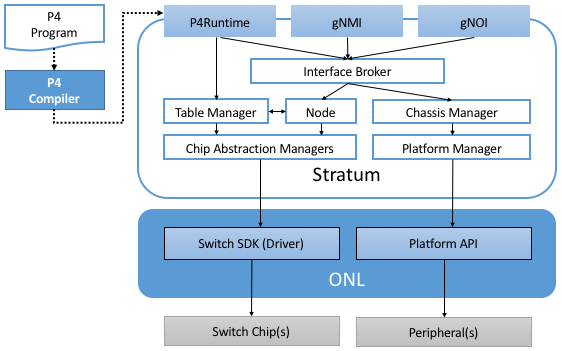
\includegraphics[width=1\linewidth]{graphics/switch-os-arch.png}
    \caption{"Thin" Switch OS architecture that is designed for vendor-agnostic. Adapted from \cite{systemsapproach}.}
    \label{fig:switch-os-arch}
\end{figure}